\chapter{Ejercicio de Autolocalización con Láser}\label{cap.laserloc}
Este capítulo recoge el proceso de elaboración y testeo de la segunda práctica creada para el entorno de aprendizaje JdeRobot-Academy. En él, se explicará el desarrollo que ha sido necesario para su infraestructura, las características de simulación bajo las que se ha creado la práctica, el nodo académico y la solución de referencia programada, así como la versión en cuadernillo Jupyter del ejercicio.

\section{Enunciado} \label{sec.enunciado}
El objetivo de esta práctica es que el alumno entre en contacto con uno de los problemas clásicos de la robótica moderna: la auto-localización. En muchos casos, es necesario para que un robot desempeñe su tarea que conozca en todo momento su posición.

Este problema se resuelve empleando alguno de los diversos algoritmos de auto-localización existentes. En concreto, este ejercicio se orienta a emplear el método del filtro de partículas, asumiendo que el robot conoce de antemano el mapa del escenario en que se va a mover. Se usará un robot aspiradora \textit{Roomba} que incorpora únicamente un sensor láser y un sensor de odometría, además de motores para poder efectuar movimientos en cualquier dirección. 

El estudiante deberá programar un algoritmo de auto-localización que permita a la aspiradora estimar su posición en un mundo del cual sólo se proporciona un mapa binario en escala. El interfaz gráfico (GUI) de esta práctica incluye distintos \textit{widgets} que facilitan la depuración, con espacios reservados para una visualización adaptada de las lecturas del sensor láser y el propio mapa del entorno, donde se marcarán en todo momento la posición del robot en el mundo, las estimaciones que se van obteniendo y otros componentes elementales que van surgiendo como salida del algoritmo mencionado. 

En este caso, el algoritmo funcionará en paralelo con la navegación, el robot puede teleoperarse o deambular autónomamente y el algoritmo de autolocalización funciona independientemente.

\section{Infraestructura desarrollada}
En este apartado se describirá el soporte que sostiene la práctica. Se comenzará describiendo el modelo de robot empleado, así como los sensores y actuadores que posee. Después, los entornos simulados y sus características, de vital importancia para la práctica, serán descritos.

\subsection{Modelo de robot de interiores con sensor láser}
El robot en el que se ha inspirado esta práctica es la aspiradora autónoma modelo \textit{Roomba} de la serie 500, que fue comercializado por la empresa iRobot. Esta aspiradora robótica está equipada con sensores varios con los que sacar conclusiones a partir del entorno y actuadores que le permiten moverse adecuadamente por el escenario. Los dispositivos \textit{Roomba} de esta serie en concreto poseen sensores infrarrojos, un sensor detector de suciedad, un sensor detector de desniveles, y cuentan además con un \textit{bumper}. No todos serán necesarios para abordar la tarea de auto-localización, aunque algunos seguirán estando disponibles en el modelo. Para la práctica se ha creado el modelo \textit{RoombaROS}, que no tiene detector de desniveles debido a que en el escenario elegido no hay escaleras o cambios de nivel entre habitaciones, y tampoco tiene detector de suciedad, puesto que no es necesario. El objetivo de la práctica era hacer énfasis en el algoritmo de navegación, de manera que de los sensores restantes sólo se usarán el de odometría, para detectar el número de veces que giran las ruedas, y el láser, para medir distancias a los obstáculos; ambos detallados más adelante. 

El robot \textit{Roomba} de la serie 500 posee una anchura de 340 milímetros, 92 milímetros de altura, y un peso de 3.6 kg. El modelo RoombaROS de JdeRobot mide aproximadamente 330 mm de ancho, 90 mm de altura, y un peso de 2.5 kg.

\begin{multicols}{2}
	\begin{figure}[H]
	\begin{center}
		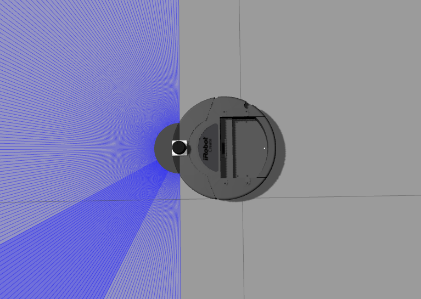
\includegraphics[width=0.3\textwidth]{figures/create.png}
		\caption{Modelo Roomba ROS}
		\label{fig.create}
		\end{center}
\end{figure}

Partiendo del modelo de la Figura 5.1, se enriquecerá el mismo para que incluya todas las interfaces de sensores y actuadores anteriores que se comunicarán a través de \textit{plugins} de ROS.
\end{multicols}
En cuanto al sensor láser, hemos utilizado un modelo ya creado llamado \textit{hokuyo} (Figura 5.2) que ya se comunica a través de \textit{ROS Messages}, el cual se ha incrustado en la parte frontal del robot.

Para implementar toda la funcionalidad anterior en la aspiradora, hemos usado los siguientes \textit{plugins}:

\begin{multicols}{2}
	\begin{figure}[H]
	\begin{center}
		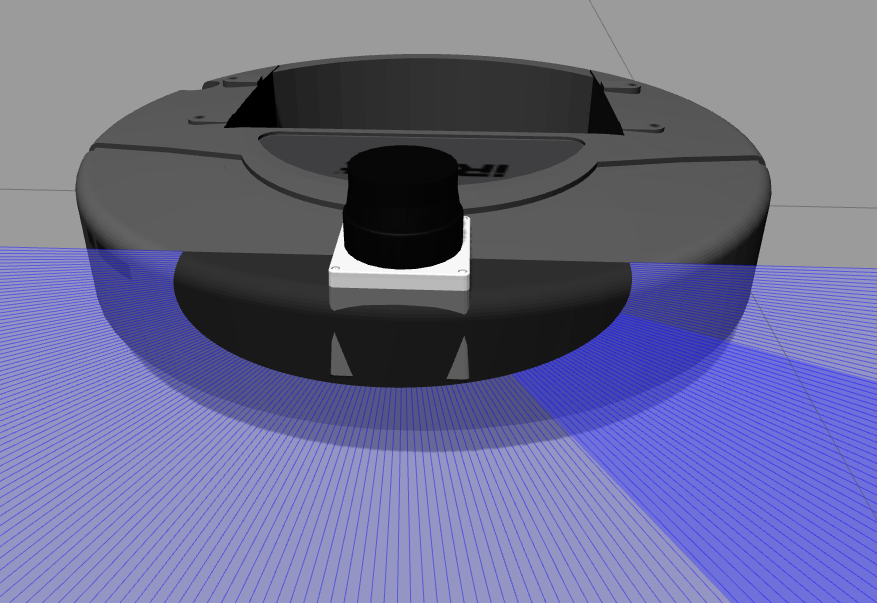
\includegraphics[width=0.3\textwidth]{figures/hokuyo.png}
		\caption{Modelo Hokuyo sobre Roomba}
		\label{fig.hokuyo}
		\end{center}
\end{figure}

\begin{itemize}
	\item \textit{libgazebo\_ros\_bumper.so} 
Para gestionar el sensor bumper
	\item \textit{libgazebo\_ros\_laser.so}  
Para recibir datos del sensor láser
	\item \textit{libgazebo\_ros\_diff\_drive.so } 
Para obtener odometría y controlar motores
\end{itemize}
\end{multicols}

Todos ellos compatibles con la versión \textit{kinetic} de ROS.

Una vez creado el modelo, basta con incluirlo en el mundo o escenario deseado para poder usarlo.

\subsubsection{Sensor láser}
En la parte frontal del robot se ha modelado un sensor láser que se utilizará en todo momento en la práctica, por lo que constituye el sensor más importante a estos efectos. 

Está compuesto por un \textit{array} de 180 medidas, que puede medir distancia alrededor de 180 grados en milímetros, con precisión de 1 grado. Su funcionamiento se basa en emitir rayos láser en todas estas orientaciones, que rebotan sobre los objetos existentes (si los hay) de manera no especular, de tal manera que al recibir el rayo devuelto se calcula la distancia al objeto según el tiempo de vuelo.

El nodo académico se encargará de recibir los datos del sensor y adaptarlos en forma de un API sencillo de utilización, para que estén accesibles desde el algoritmo que el alumno debe programar. Se ha construido un \textit{parser} para la práctica que agrupa los datos en forma de \textit{array} de 180 distancias, donde el índice es el ángulo de proyección del haz del láser.
 
\subsubsection{Sensor Odométrico}
En ésta práctica jugará un papel importante el saber cuánto se ha desplazado el robot en un intervalo, dado que servirá para desechar o evolucionar datos involucrados en el algoritmo de auto-localización que explicaremos en 5.4.1. Ésta es precisamente la función de la odometría: el uso de sensores de movimiento para determinar el cambio de posición del robot en relación con una posición conocida. Si el robot conoce el diámetro de sus ruedas, simplemente le basta con contar el número de revoluciones de las mismas para determinar qué tan lejos ha viajado. Normalmente, el conteo de vueltas se realiza a través de \textit{encoders}, que emiten un número fijo de pulsos por revolución, siendo éstos los registrados por el software.

Así, el sentido de giro y el número de vueltas que da cada rueda nos ayudará a saber en qué dirección se ha movido el robot, y cuánta distancia ha recorrido.

\subsection{Escenario de casa asimétrica} 
Dado que la aspiradora necesita un entorno acotado para determinar su localización (el láser tiene un alcance limitado), se ha creado un modelo para que la aspiradora navegue en él.
Hemos partido del diseño \textit{house\_int2} que utiliza la práctica \textit{Vacuum Cleaner} de JdeRobot-Academy como punto de partida. Este modelo se puede ver en la Figura 5.3:

\begin{figure}[H]
  \begin{center}
    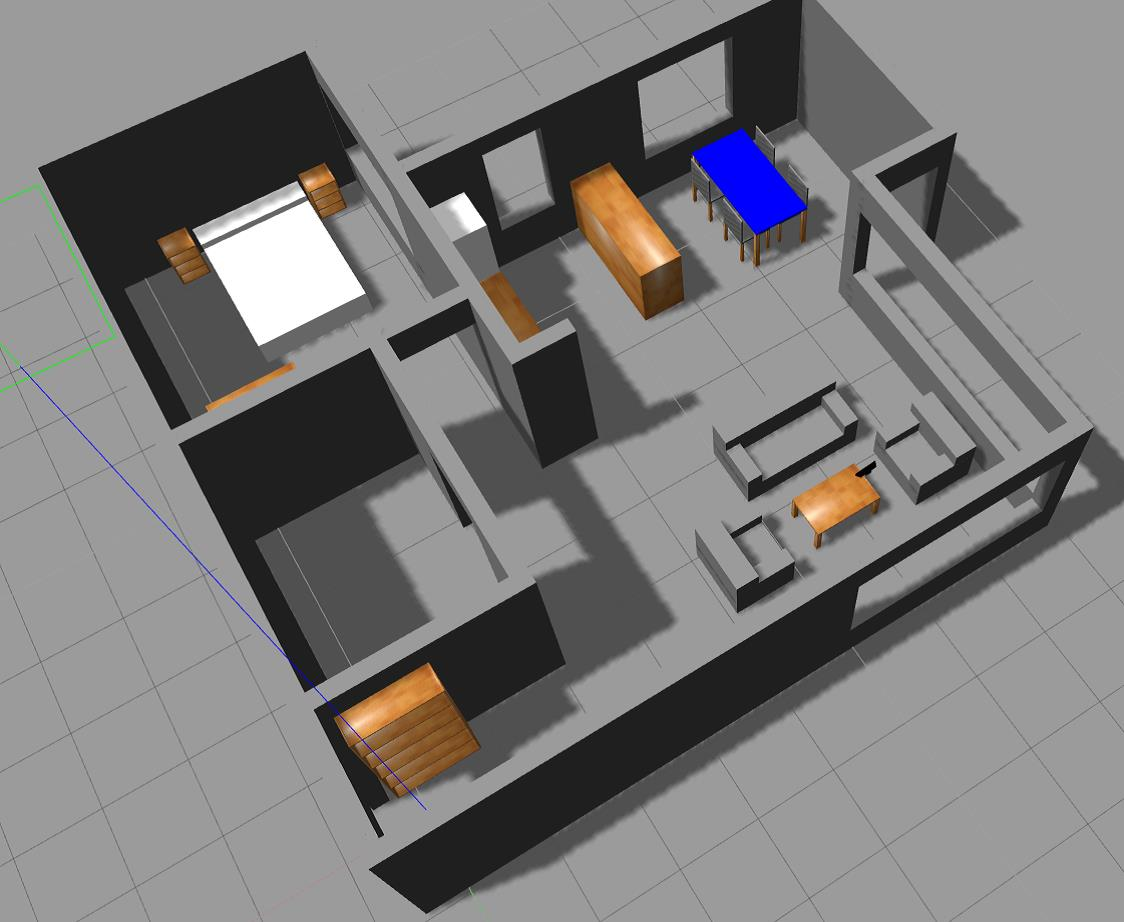
\includegraphics[width=0.75\textwidth]{figures/houseint.jpg}
		\caption{Modelo house\_int2}
		\label{fig.houseint}
		\end{center}
\end{figure}

Las razones bajo la elección de este modelo son:

\begin{itemize}
	\item[--] Entorno acotado por paredes, ideal para obtener lecturas del sensor láser representativas.
	\item[--]	Abundantes obstáculos, lo cual favorece la diferencia entre lecturas en cada punto de la casa.
	\item[--]	Malla de colisiones bien definida, importante cuando se quiere que el robot navegue por la casa sin la aparición de sucesos extraños, como objetos voladores al colisionar con ellos. 
\end{itemize}

Aún con todo ello, este modelo emplea elementos de difícil modelado en una imagen 2D (necesaria para establecer el mapa del mundo), como puede ser la mesa y las sillas: cada pata debía tener el tamaño exacto a escala y estar en la posición adecuada para no obtener procesados erróneos. La zona bajo la cama también resultó un problema. 

Dadas las múltiples ventajas que presenta, se ha creado un nuevo modelo, basado en el anterior, que sustituye todos los elementos difíciles de modelar por paredes, claramente definidas y representadas, mucho más fáciles de modelar en un mapa. Al nuevo mundo que incluía este modelo y el modelo de aspiradora se le ha llamado \textit{Asymmetric-Easy-To-Model.world} (Figura 5.4):

\begin{figure}[H]
  \begin{center}
    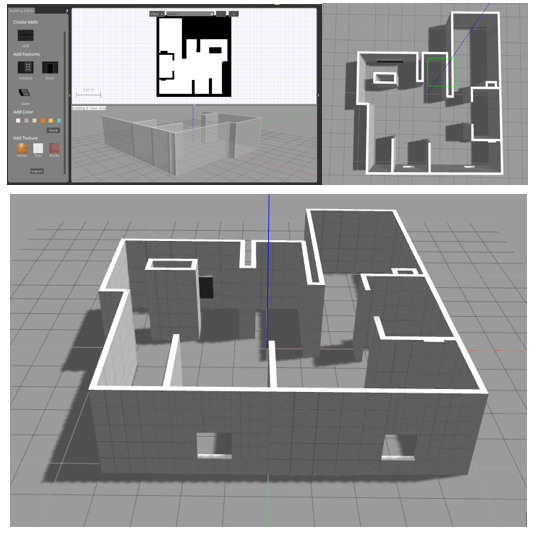
\includegraphics[width=0.95\textwidth, height=12cm]{figures/modeloasymmetric.png}
		\caption{Modelo Asymmetric-Easy-To-Model}
		\label{fig.modeloasymmetric}
		\end{center}
\end{figure} 

\subsection{Modelo de nave simétrica}
El modelo anterior es el caso más común en el que nos encontramos con el problema de la auto-localización, no obstante, también existen lugares donde las formas se repiten o las superficies límite son iguales o similares en distintas orientaciones. Es por eso que hemos decidido crear el mundo de Gazebo \textit{Choso.world}, el cual es una habitación cuadrada con sólo dos elementos, que ocupan muy poco espacio y por tanto pasan desapercibidos en la mayoría de casos. Este modelo se puede ver en la siguiente imagen (Figura 5.5):

\begin{figure}[H]
  \begin{center}
    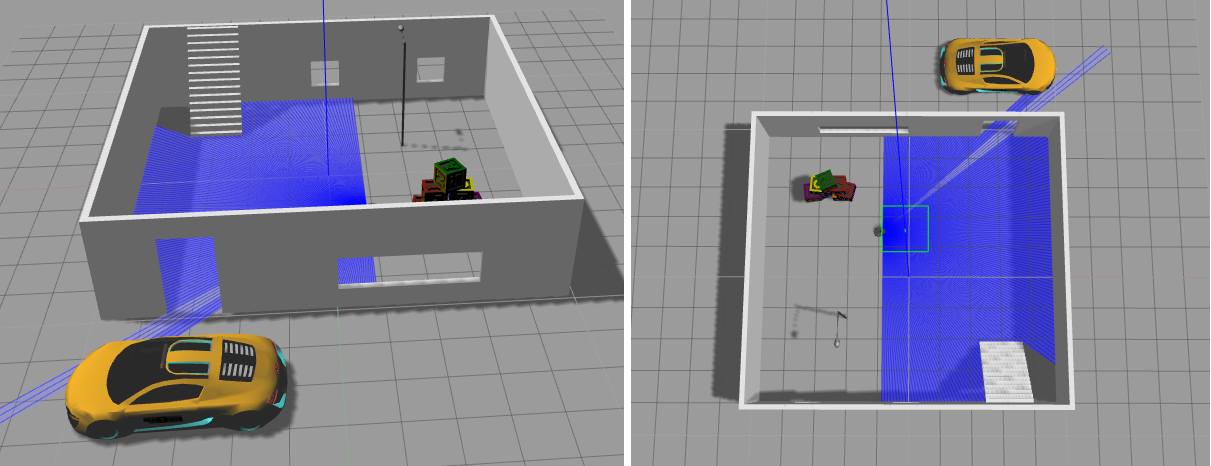
\includegraphics[width=0.96\textwidth]{figures/chosoworld.png}
		\caption{Modelo Choso}
		\label{fig.choso}
		\end{center}
\end{figure}

Introduciremos al robot en este modelo con fines de experimentación y verificación del comportamiento del algoritmo de autolocalización.

\subsection{Ficheros de configuración}
Incorporando los dos modelos involucrados (\textit{Asymmetric-Easy-To-Model} y \textit{RoombaROS}) y algunas fuentes de luz como el sol, luz ambiente y algunas sombras, se crea el mundo principal en el que abordar la práctica: \textit{Asymmetric-Easy-To-Model.world} (Figura 5.6). Debido a la extensión del fichero de descripción del mundo, sólo incluimos a continuación una parte del mismo para observar su aspecto:

\begin{figure}[H]
  \begin{center}
    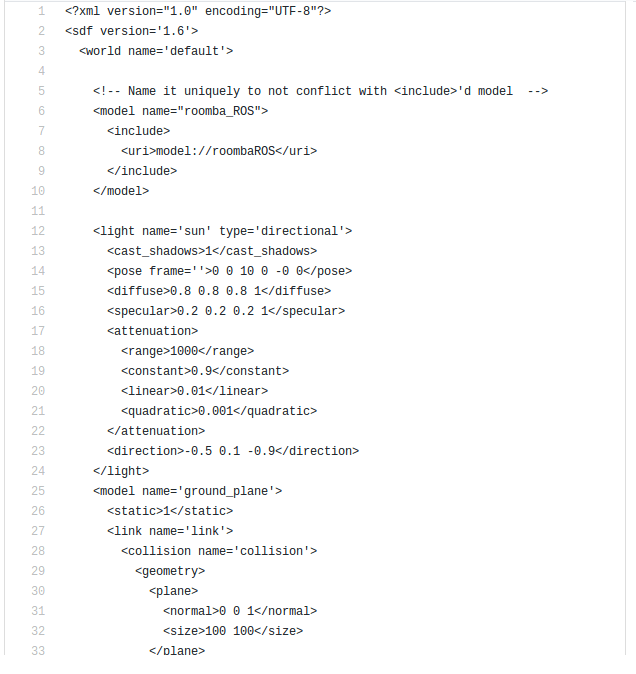
\includegraphics[width=0.98\textwidth]{figures/codeworld.png}
		\caption{Código del mundo}
		\label{fig.codeworld}
		\end{center}
\end{figure}

En él, se puede ver la combinación del modelo de robot creado y de los parámetros de física, aspecto, iluminación y posición que componen el mundo.

\section{Nodo Académico}

\begin{figure}[H]
\begin{center}
	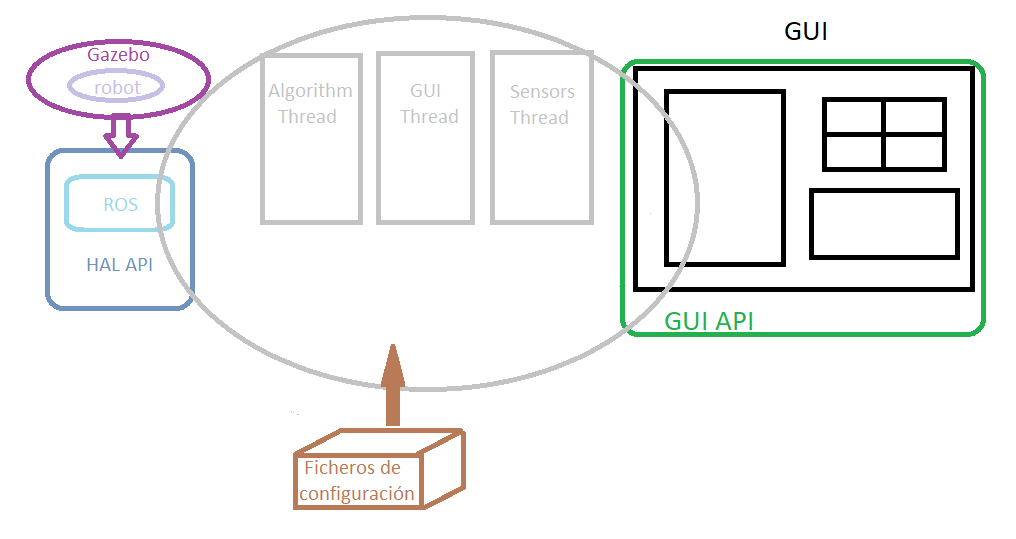
\includegraphics[width=0.95\textwidth]{figures/nodoacademicoll.png}
	\caption{Diseño de Nodo académico de Laser Loc}
	\label{fig.nodoacademicoll}
	\end{center}
\end{figure} 

El componente académico que se ha preparado para esta práctica (Figura 5.7) recoge toda la funcionalidad para ayudar al alumno a enfrentarse a ella y resolverla con éxito. Estas son las piezas que conforman el componente y que quedan resueltas a través de él:  

\begin{enumerate}[label=\alph*)]
	\item Ofrece acceso a todas las interfaces que el robot posee, tanto sensores como actuadores, en forma de métodos simples. Oculta el \textit{middleware} de comunicaciones.
	\item Ofrece una interfaz gráfica al usuario que le ayuda a depurar su código.
	\item Incluye código auxiliar, como \textit{parsers} o constructores de objetos, que no son parte del algoritmo a realizar, pero que sirven de ayuda para hacer la tarea más sencilla.
\end{enumerate}

El componente pone la base que el estudiante culmina incluyendo su código en el método \textit{execute} del fichero \textit{MyAlgorithm.py}, siempre realizando las pruebas que considere oportuno para pulir su solución.

\subsection{Arquitectura software}
El componente se ha dividido en distintos hilos para favorecer la simultaneidad de ejecución de distintas tareas clave. En un principio, el componente sólo contaba con dos hilos básicos de ejecución, pero el diseño final elegido es con tres, de modo que se agiliza su funcionamiento:

\begin{itemize}
  \renewcommand{\labelitemi}{$\to$}
	\item Hilo de algoritmo: se encarga del refresco de la ejecución del algoritmo, ya que este se ejecuta de modo iterativo o cíclico. El tiempo de refresco es importante, dado que el algoritmo necesario para solventar la práctica es bastante sensible a pequeños cambios en las lecturas, que deben desencadenar correcciones en la ejecución. Por ello, el tiempo de refresco es de 10 ms.
	\item Hilo de la interfaz gráfica de usuario (GUI): Este hilo es el encargado de actualizar la interfaz gráfica y los \textit{widgets} incorporados en ella. El intervalo de actualización de la interfaz debe ser pequeño, de tal manera que los cambios en los sensores o en el mapa puedan ser representados en tiempo real. Por ello, se ha fijado el tiempo de refresco a 20 ms.
	\item Hilo de sensores: el tercer hilo se ha añadido para actualizar los datos de los sensores y los actuadores a través de las interfaces que correspondan (ROS). El tiempo de refresco de este hilo es muy importante, dado que un intervalo largo radicaría en lecturas desactualizadas de los sensores. Por ello, dicho tiempo también se ha fijado en 20 ms.
\end{itemize}

Con todo ello, el nodo dispone la interfaz de usuario con algunos elementos de depuración (accesibles a través de un API descrito en 5.3.2 y 5.3.3) para que el usuario se centre en el algoritmo a escribir. La manera de integrar dicho algoritmo en el nodo para que llegue al robot también es tarea del componente académico, por lo cual se reserva un espacio concreto para que el alumno inserte la lógica, debidamente indicado en el fichero de instrucciones incluido (\textit{README.md}).

\subsection{Interfaz de sensores y actuadores y código auxiliar}
El nodo ofrece un API de sensores y actuadores al programador, además de un API específico auxiliar para la práctica en el que se encontrarán otros métodos e incluso variables disponibles para facilitar la tarea. En cuanto al API del robot, tenemos:

\begin{itemize}
	\item \textit{self.sensors.motors.sendVelocities(vel)}: Para enviar comandos de velocidad a través de:
    \begin{itemize}[label={$\diamond$}]
			\item \textit{vel = CMDVel()}: constructor de comandos de velocidad
       \item \textit{vel.vx = valor}: velocidad lineal
       \item \textit{vel.az = valor}: velocidad angular
    \end{itemize}
    \item \textit{self.sensors.laserdata} o \textit{self.gui.getLaserData()}: dos posibilidades equivalentes para obtener los datos láser.
    \item \textit{self.parse\_laser\_data(laser)}: Para transformar los datos láser en una estructura más fácilmente manejable.
		\item \textit{self.pose3d.getPose3d().x}, \textit{self.pose3d.getPose3d().y}, \textit{self.pose3d.getPose3d().yaw}: para obtener los datos de posición y orientación del robot.
\end{itemize}

Por otro lado, el nodo académico incluye cierto código auxiliar en el cual el estudiante puede apoyarse
para desarrollar su solución. Este código simplifica ese desarrollo y su interfaz de programación es:

\begin{itemize}
	\item ||\textbf{Clase Particle}||: \textit{Particle(x, y, yaw, prob, self.map.robotAngle)}: Constructor de partículas.
	\item \textit{img = self.map.pixmap.toImage()}: para obtener la imagen (mapa) del interfaz.
	\item \textbf{(variable)} \textit{self.particleClicked}: almacena la última partícula sobra la que se ha hecho click en el GUI. 
	\item \textit{self.map.map2pixel((x,y))}: obtiene el pixel correspondiente a las coordenadas (x,y).
	\item \textit{self.map.pixel2map((px,py))}: obtiene las coordenadas reales asociadas al pixel [px,py] del mapa.
\end{itemize}

Con ello y una forma de representación de las partículas involucradas en el algoritmo, todo lo necesario queda a disposición del alumno para comenzar la tarea. 

\subsubsection{Partículas}
El elemento principal en el que se basa el algoritmo que se debe emplear en la solución son las partículas, las cuales ya hemos mencionado en el desarrollo de este capítulo. Estas partículas no son más que puntos en el espacio 2D en los que el robot se proyecta a sí mismo, es decir, posiciones y orientaciones que el robot puede ocupar y tomar en el escenario. Por ello, cada partícula consta de:

\begin{itemize}
  \renewcommand{\labelitemi}{$\to$}
	\item Un vector de coordenadas (x, y, z) que representa su posición en el espacio. La coordenada z se fija siempre a 0, dado que el escenario no contiene desniveles.
	\item Un atributo de orientación, que representa su rotación con respecto al mapa. 
	\item Un valor de probabilidad, que almacena el valor numérico obtenido al comparar el láser de la partícula con la lectura real.
\end{itemize}

A fin de organizar el código, se ofrece al programador la clase \textit{Particle}¸ la cual actúa como constructor de partículas, asociando a cada una sus correspondientes características accesibles como atributos de un objeto Python:

\begin{figure}[H]
	\begin{center}
		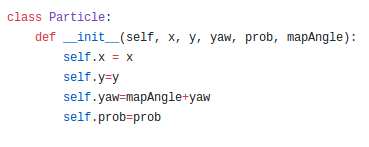
\includegraphics[width=0.6\textwidth]{figures/claseparticle.png}
		\label{fig.claseparticle}
		\end{center}
\end{figure}

\subsection{Interfaz gráfica y uso desde código}
La interfaz gráfica de usuario (GUI) se emplea para representar información que ayuda a resolver el algoritmo planteado, lo cual resultará vital en el camino hacia la resolución de la misma. Se ha construido a través de PyQt5, y se encarga de mostrar la salida de la ejecución del algoritmo en cada instante, ideal para depurar y observar su evolución.

\begin{figure}[H]
  \begin{center}
    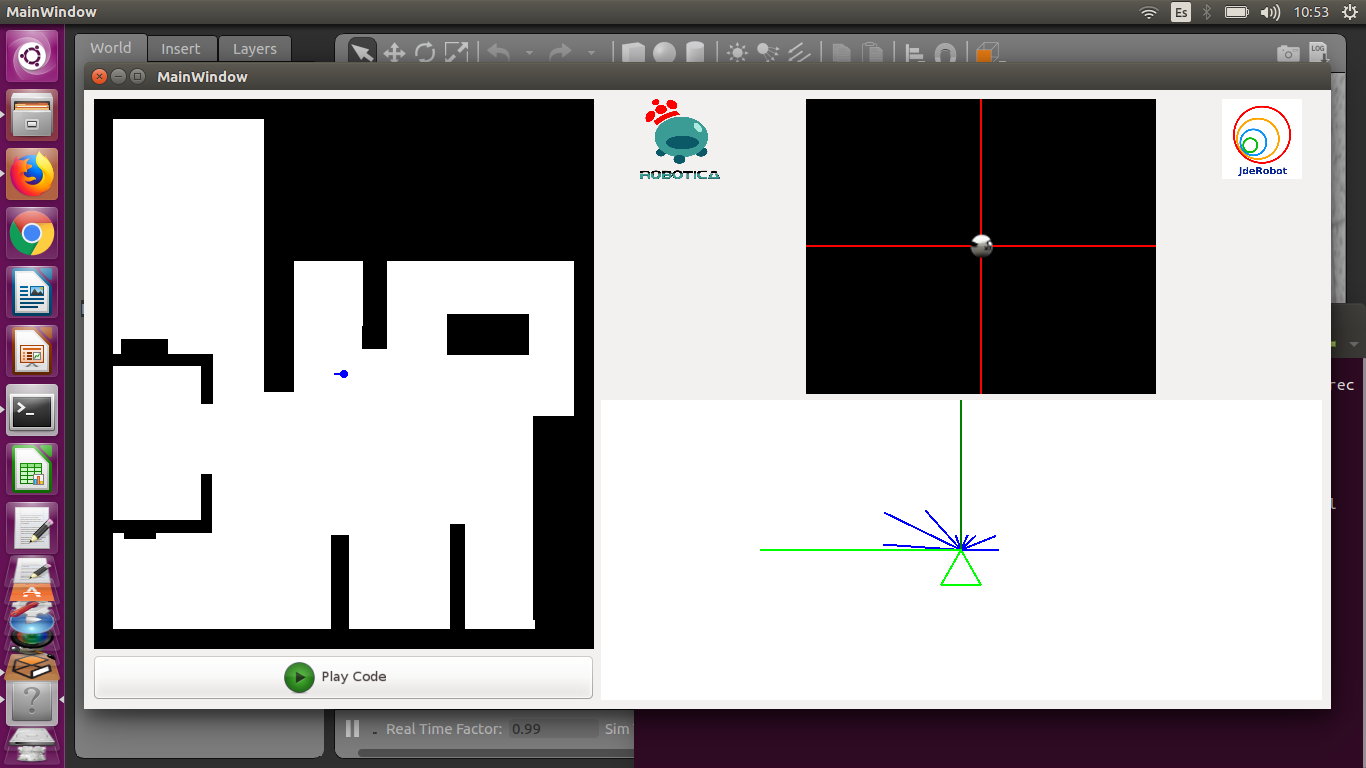
\includegraphics[width=0.98\textwidth]{figures/llgui.png}
		\caption{Interfaz Gráfica Laser Loc}
		\label{fig.llgui}
		\end{center}
\end{figure}

Esta GUI (Figura 5.8) está formada por 3 \textit{widgets} para el control y visionado del comportamiento del robot. El primero de ellos, situado a la izquierda, es quizás el más importante, pues muestra al programador el mapa binario que el robot utiliza para realizar cálculos pertinentes para llevar a cabo su auto-localización. También muestra información gráfica con la que éste no cuenta: las sucesivas generaciones de partículas que surgen del algoritmo evolutivo. En el mapa se ven reflejados los obstáculos (zonas negras), las zonas libres (espacio en blanco), la posición y orientación del robot en el espacio dado (a través de un punto azul), la evolución de las partículas e incluso las trayectorias.
 
El segundo de los elementos del interfaz, situado en la parte superior derecha, es el clásico teleoperador, para controlar la posición del robot y su rotación a través de órdenes de velocidad lineal y angular. Esto facilita el proceso de depuración y sirve de apoyo en los primeros pasos hacia la solución.

Por último, el espacio inferior derecho se ha reservado para la representación de las lecturas que ofrece el láser del robot en cada momento, y también para dibujar de manera aproximada el cálculo de láser teórico que el robot hace de cada partícula.

En la parte inferior se ha incluido un botón para ejecutar el algoritmo y pararlo cuando sea necesario, deteniendo todas las representaciones y el movimiento del robot. 

Para hacer uso de la funcionalidad de depuración que ofrece el interfaz gráfico, se ha dispuesto un interfaz de programación con los siguientes métodos:

\begin{itemize}
	\item \textit{self.setParticles([p1,p2,p3,...])}: Representa una lista de partículas en el GUI.
	\item \textit{self.setEstimation(particle)}: Para mostrar una estimación en el interfaz.
	\item \textit{self.paintTheoricalLaser(theoricalLaser)}: para representar un láser en la interfaz.
\end{itemize}

\subsubsection{Gráfica de los láseres Real y Teórico}
Uno de los elementos de visualización que incluye la práctica es la posibilidad de ver de forma gráfica los datos que ofrece el sensor láser, así como una representación de los haces láser de cada partícula calculados a partir de la lectura que ofrecería el robot en el caso de que su posición y orientación coincidiesen con los de esta. Así, lo que se representa es lo siguiente:

\begin{enumerate}
	\item \textbf{- Láser Real}
	\begin{figure}[H]
		\begin{center}
			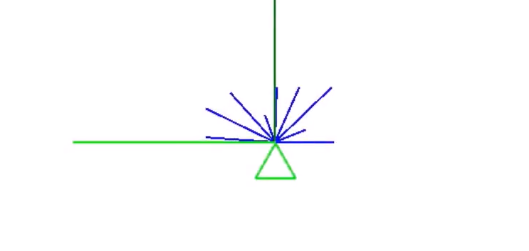
\includegraphics[width=0.65\textwidth]{figures/laserreal.png}
			\caption{Laser Real}
			\label{fig.laserreal}
			\end{center}
	\end{figure}
Dado que las lecturas utilizadas para esta práctica están formadas por 9 haces en total (uno cada 20º con respecto a la normal de la orientación del robot), lo que se representa es un conjunto de segmentos cuya longitud se corresponde con la distancia (a escala 50:1) al primer obstáculo en la dirección marcada por el ángulo del haz (Figura 5.9). Las medidas del láser constan de 180 pares de valores, y su reducción a los 9 utilizados se describirá en 5.4.2. Los datos del sensor se analizan convenientemente antes de ser representados, y la representación es en todo caso relativa al propio robot.
\item \textbf{- Láser Teórico}
	\begin{figure}[H]
		\begin{center}
			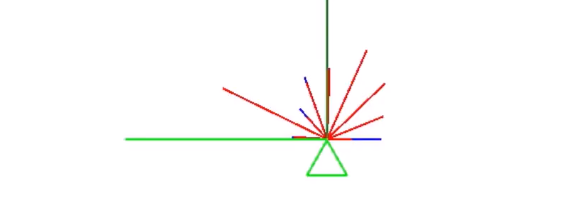
\includegraphics[width=0.65\textwidth]{figures/laserteorico.png}
			\caption{Laser Teórico}
			\label{fig.laserteorico}
			\end{center}
	\end{figure}
Como veremos más adelante, para cada partícula involucrada en el algoritmo se deberá calcular un “láser teórico” (Figura 5.10), es decir, la lectura que se obtendría en el sensor en el supuesto de que el robot ocupase la posición de dicha partícula y compartiese su orientación. En la representación se muestra la superposición de ambos datos láser: el real en azul y el teórico en rojo, de manera que en todo momento se puede comprobar si una partícula ofrece una lectura similar a la del robot o no. 

Dado que el algoritmo se compone de muchas partículas, para activar la representación del láser teórico de una partícula determinada bastará con hacer click sobre ella en el \textit{widget} que contiene el mapa de referencia.
\end{enumerate}

\subsubsection{Mapa de Referencia}
El elemento gráfico vital es el mapa que robot utiliza para hacer cálculos sobre su entorno. Este mapa es una imagen con sólo dos valores posibles para cada pixel: blanco y negro. Esto facilita las tareas de procesado. El robot se basa en dicho mapa para realizar el cálculo de los datos teóricos láser, llevando a cabo un trazado de rayos sobre la imagen. 

Este mapa emplea una codificación de color para expresar visualmente la probabilidad de cada partícula, como el que se muestra en la Figura 5.11. Así, cada partícula se representará con un color dentro de este rango, en función de sus posibilidades de ser la posición real en la que se encuentra el robot.

\begin{figure}[H]
	\begin{center}
		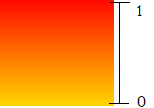
\includegraphics[width=0.3\textwidth]{figures/gradcolor.png}
		\caption{Codificación de color}
		\label{fig.gradcolor}
		\end{center}
\end{figure}

Además, en el mapa se mostrarán:
\begin{itemize}
	\item[--] La posición real del robot, también representada en forma de partícula, utilizará un color azul oscuro en todo momento
	\item[--] Las estimaciones que el robot hará de su posición se representarán en azul claro.
\end{itemize}

Por último, este lienzo también superpondrá al mapa la trayectoria real que el robot sigue en todo momento representada en negro, y la trayectoria estimada por el robot para localización en movimiento, representada también en azul claro, como se ve en la Figura 5.12:

\begin{figure}[H]
	\begin{center}
		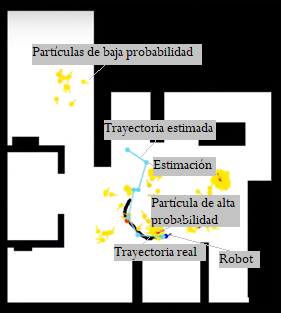
\includegraphics[width=0.5\textwidth]{figures/mapareferencia.png}
		\caption{Mapa de referencia}
		\label{fig.mapareferencia}
		\end{center}
\end{figure}

\subsubsection{Trayectorias}
En cuanto a las trayectorias que se representan en el gráfico, cabe decir que la ruta real está formada por las últimas 100 posiciones diferentes que ha ocupado el robot para su representación, de manera que se modifica con las sucesivas iteraciones. Sirve como apoyo para pulir el comportamiento del algoritmo, ya que el programador podrá compararla en todo momento con la trayectoria que su propio algoritmo de localización va estimando. Su representación es automática y se encarga la interfaz del nodo académico.

Por otro lado, la trayectoria estimada es obtenida a través de la unión de las distintas estimaciones de posición que el algoritmo del robot hace a lo largo del tiempo. Se ha dotado al componente con un API para el establecimiento de estimaciones a visualizar en la gráfica, con lo cual se puede hacer un seguimiento del comportamiento del algoritmo a largo plazo:

\hspace{0.32\linewidth} \textit{self.setEstimation([x,y])}
 
\subsection{Comunicaciones con sensores y actuadores}
La práctica debe ser auto-contenida, de manera que el nodo académico debe icluir en su fichero principal (\textit{laser\_loc.py}) todo lo necesario para establecer y mantener la comunicación con el robot, inicializando los distintos nodos de comunicación con sensores y actuadores y suscribiendose o publicando en un \textit{topic} adecuado para cada interfaz del robot. Además, debe realizar la conversión entre los mensajes recibidos y los datos que el nodo académico puede manejar. 

Por tanto, dicho fichero debe contener:
\begin{enumerate}
	\item El código necesario para conectar con cada nodo del robot, para lo cual se usan sentencias tipo:
	\begin{figure}[H]
	\begin{center}
		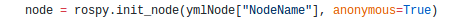
\includegraphics[width=0.75\textwidth]{figures/initnode.png}
		\label{fig.initnode}
		\end{center}
	\end{figure}
	\item La suscripción de cada nodo inicializado a su correspondiente \textit{topic} de ROS, es decir, a su bus de intercambio de mensajes en el cual el driver encargado del control del nodo (ya sea sensor o actuador) publica o recibe mensajes con cierta forma:
	\begin{figure}[H]
	\begin{center}
		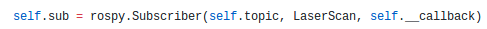
\includegraphics[width=0.75\textwidth]{figures/subscriberlaser.png}
		\label{fig.subscriberlaser}
		\end{center}
	\end{figure}
	\hspace{0.48\linewidth}o
	\begin{figure}[H]
	\begin{center}
		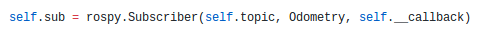
\includegraphics[width=0.75\textwidth]{figures/subscriberodometry.png}
		\label{fig.subscriberodometry}
		\end{center}
	\end{figure}
	\item La transformación de los mensajes que se intercambian por la red a la estructura utilizada por el nodo de la práctica:
	\begin{figure}[H]
	\begin{center}
		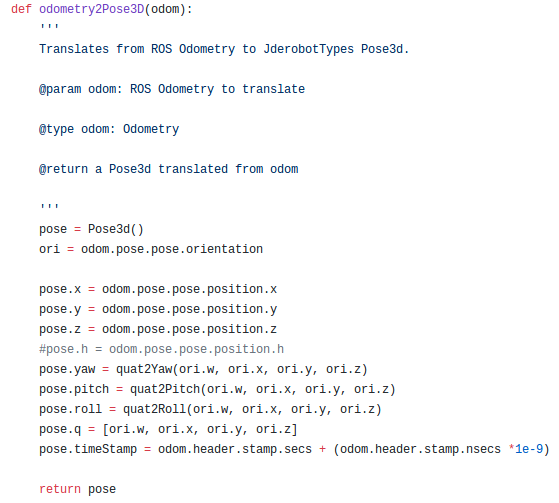
\includegraphics[width=0.60\textwidth]{figures/odom2pose.png}
		\label{fig.odometry2pose}
		\end{center}
	\end{figure}
\end{enumerate}

Para todo ello, el fichero principal amplía su funcionalidad con una serie de clases que se encargan de la construcción de objetos que tengan en cuenta todas las especificaciones anteriores.

\subsection{Fichero de configuración}
El único elemento externo que el nodo académico necesita es un fichero de configuración que recoja los \textit{endpoints} que las interfaces de los sensores y actuadores descritos en 5.3.2 utilizan para publicar la información o recibirla del nodo. Este archivo tiene extensión \textit{.yml}, lo cual implica que debe cumplir las especificaciones del formato de serialización de datos YAML. Para esta práctica en concreto, añadimos además la configuración necesaria para establecer el mapa binario de referencia del robot.

La asociación entre cada nodo y su \textit{topic} se ha de facilitar también en el fichero a la hora de ejecutar. Tiene el siguiente aspecto (Figura 5.13):

\begin{figure}[H]
	\begin{center}
		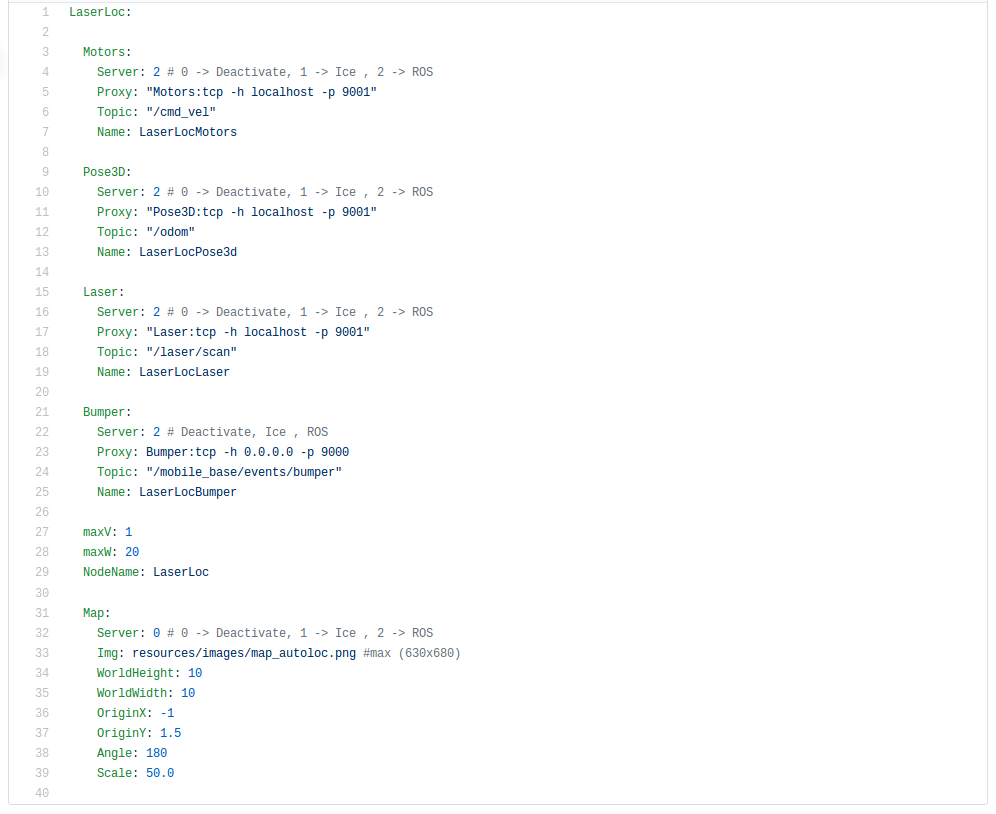
\includegraphics[width=0.98\textwidth]{figures/llymlfinal.png}
		\caption{Fichero de configuración YAML con interfaces de ROS}
		\label{fig.llymlfinal}
		\end{center}
\end{figure}

Vemos que la información del mapa cuenta con atributos como el tamaño, la escala o el \textit{path} que conduce a la imagen binaria. Por último, se establecen las velocidades máximas de tracción y rotación en base a las necesidades de la práctica. 

\section{Solución de referencia}
Para esta práctica no es adecuado incluir también un algoritmo de pilotaje, pues se dispone de un teleoperador y el foco está en la autolocalización que se ejecuta de modo independiente mientras el robot se mueve (teleoperado o autónomo). Construiremos una solución que se establecerá como solución de referencia en el fichero \textit{MyAlgorithm.py} que tiene naturaleza iterativa, de manera que en cada iteración se obtiene datos de los sensores, se procesan y se evoluciona el algoritmo de localización. El código a escribir irá de nuevo a parar al método \textit{execute}, el cual ejecuta la lógica de manera cíclica en el \textit{thread} de algoritmo y computación.

\subsection{Fundamentos de autolocalización basada en filtros de partículas}
El filtro de partículas aplicado al problema de la autolocalización de robots consiste en mantener un conjunto muestral de posibles posiciones y calcular la probabilidad de cada una. Mediante remuestreo estadístico, estas posiciones acaban convergiendo hacia la posición correcta del robot. El número reducido de muestras (comparado con el de la localización probabilística basada en rejillas) hace que se minimicen los costes computacionales y que el algoritmo sea escalable a grandes entornos. Se trata de un filtro bayesiano recursivo en el que el conjunto de muestras
\begin{equation}
\{x_{i},P(x_{i})\}, i = 1..n,
\end{equation} estaría formado por coordenadas de posición y orientación
\begin{equation}
x_{i} = (x, y, \theta),
\end{equation} inicialmente escogidas al azar sobre el escenario, que emplea su probabilidad P(xi) para ir seleccionando aquellas posiciones más probables. Cada muestra se denomina “partícula”, y el objetivo es conseguir que la nube de partículas converja en la posición real del robot. En cada iteración del algoritmo se evoluciona a una nueva población a partir de la anterior, la cual está formada por “hijos” de partículas que tenían alta probabilidad en dicha población anterior. El algoritmo se realiza en tres pasos que se ejecutan siempre y de forma iterativa:

\begin{itemize}
	\item \textbf{ Modelo de movimiento}: se desplazan las muestras $(\Delta r, \Delta\theta)$, equivalente al desplazamiento efectuado por el robot desde la última vez que se incorporó el movimiento del mismo. Esto permite incorporar información de desplazamiento si se dispone de ella. 
	\item \textbf{Modelo de observación}: se calculan las nuevas probabilidades de todas las muestras a partir de la lectura del sensor láser. Se ha de ajustar una función de salud que se encargue de asociar probabilidades altas a aquellas zonas compatibles con la lectura del láser real y bajar la de las zonas incompatibles. 
	\item \textbf{Remuestreo}: se genera una nueva población a partir de la anterior siguiendo el algoritmo de la ruleta (Figura 5.14), que consiste en girar la ruleta tantas veces como hijos queremos generar. Cada partícula tiene un sector proporcional a su probabilidad en la ruleta, de manera que si el valor está incluido en el sector de una partícula concreta, esta genera un hijo “idéntico” en la siguiente población.
\end{itemize}

\begin{figure}[H]
	\begin{center}
		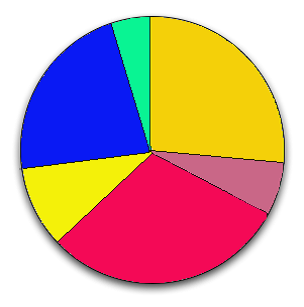
\includegraphics[width=0.3\textwidth]{figures/ruleta.png}
		\caption{Algoritmo de la Ruleta}
		\label{fig.ruleta}
		\end{center}
\end{figure}

Debajo de este modelo existen muchos parámetros relevantes para la implementación.

\begin{figure}[H]
\begin{center}
	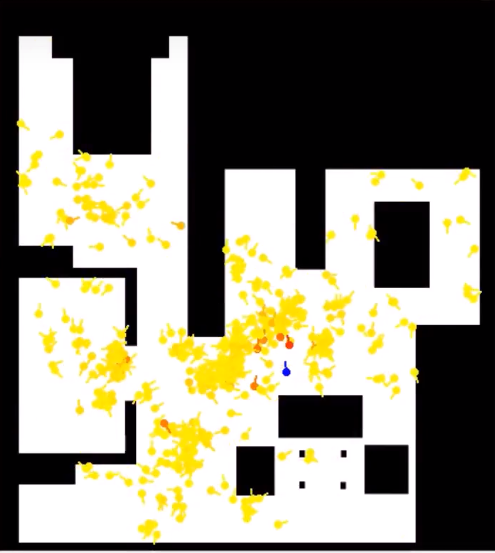
\includegraphics[width=0.4\textwidth]{figures/modeloobsv.png}
	\caption{Ejemplo de modelo de observación}
	\label{fig.modeloobsv}
	\end{center}
\end{figure}
La figura superior (Figura 5.15) muestra un ejemplo de este modelo de observación, en el cual las partículas más lejanas a la posición del robot y en distinta orientación toman valores más bajos de probabilidad representados con un color más claro (amarillo), mientras que las cercanas a la posición real toman un valor más alto, representado en un color intenso (rojo). El cálculo del “láser teórico” es lo que permite asignar a cada una su probabilidad. Para obtenerlo, emplearemos trazado de rayos sobre el mapa, tirando una línea recta en el espacio bidimensional euclidiano desde la posición de cada partícula en la imagen hasta el punto donde se encuentre el máximo de distancia que puede abarcar el láser en las 9 direcciones que componen la lectura láser. En esta recta se va comprobando cada cierta distancia (paso $\lambda$) si el color del píxel es blanco (espacio libre) o negro (obstáculo), en cuyo caso se obtiene el punto en el que rebotaría el haz láser. Con ello, y conociendo la escala del mapa dado, obtenemos una distancia para cada haz que representa la que se obtendría en el mundo si el robot ocupase esa posición. Así, 
\begin{equation}
X_{obstaculo} = (PX_{partícula} + \lambda*cos(\alpha_{haz}))*escala
\end{equation}
\begin{equation}
Y_{obstaculo} = (PY_{partícula} + \lambda*sin(\alpha_{haz}))*escala
\end{equation}
\begin{equation}
Distancia = \sqrt{(X_{obstaculo}-X_{partícula})^2+(Y_{obstaculo}-Y_{partícula})^2}
\end{equation}

Con esta distancia de cada haz, basta con compararla con la distancia observada por el sensor homólogo, con lo cual se obtendrá un error (error = LaserReal- LaserTeórico). Sólo es necesario acumular este error en cada orientación para asignar posteriormente una probabilidad. Cuanto menor error, las lecturas son más parecidas y se asignará la mayor probabilidad.

Por otro lado, el modelo de movimiento es de gran importancia para descartar información inservible y revalidar información adecuada. Se incorpora el movimiento del robot a la generación de partículas en coordenadas polares $(\Delta r, \Delta\theta)$, para lo cual: 

\begin{equation}
\Delta x = x_{t} - x_{t-1}
\end{equation}
\begin{equation}
\Delta y = y_{t} - y_{t-1}
\end{equation}
\begin{equation}
\Delta\theta = \theta_{t} - \theta_{t-1}
\end{equation}
\begin{equation}
\Delta r = \sqrt{(\Delta x)^2+(\Delta y)^2}
\end{equation}

Bastará con sumar el incremento a la posición de cada partícula de modo consecuente con la orientación de la partícula (Figura 5.16), o más en concreto con el ángulo que forma ésta con respecto a la orientación del robot.

\begin{figure}[H]
\begin{center}
	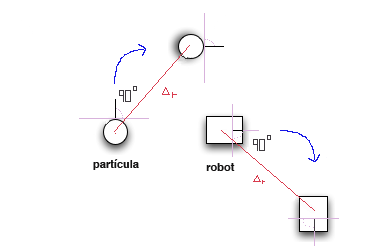
\includegraphics[width=0.4\textwidth]{figures/orientacionrelativa.png}
	\caption{Orientación Relativa}
	\label{fig.orientacionrelativa}
	\end{center}
\end{figure}

Hemos decidido aplicar geometría y trigonometría para materializarlo. En primer lugar, se construye una recta que pase por las coordenadas de la partícula $(x_{0},y_{0})$ a la cual se le va a sumar el movimiento. Esta recta se regirá por el vector de dirección creado a partir de la orientación de la partícula resultante al añadir el incremento angular:

\begin{equation}
a = cos(\theta_{0} + \Delta\theta)
\end{equation}
\begin{equation}
b = sin(\theta_{0} + \Delta\theta)
\end{equation}
\begin{equation}
y = y_{0} + \dfrac{b}{a} * (x-x_{0})
\end{equation}

Conociendo la distancia recorrida $(\Delta r)$, calculamos la coordenada x del nuevo punto al cual ha de desplazarse la partícula (y luego la coordenada y con la ecuación de la recta):

\begin{equation}
\Delta r = \sqrt{(x-x_{0})^2 + ((y_{0} + \dfrac{b}{a} * (x-x_{0}))-y_{0})^2} \Rightarrow x\, del\, nuevo\, punto
\end{equation}

Una vez hecho, ante un movimiento del robot, se tiene lo que se muestra en la Figura 5.17:

\begin{figure}[H]
\begin{center}
	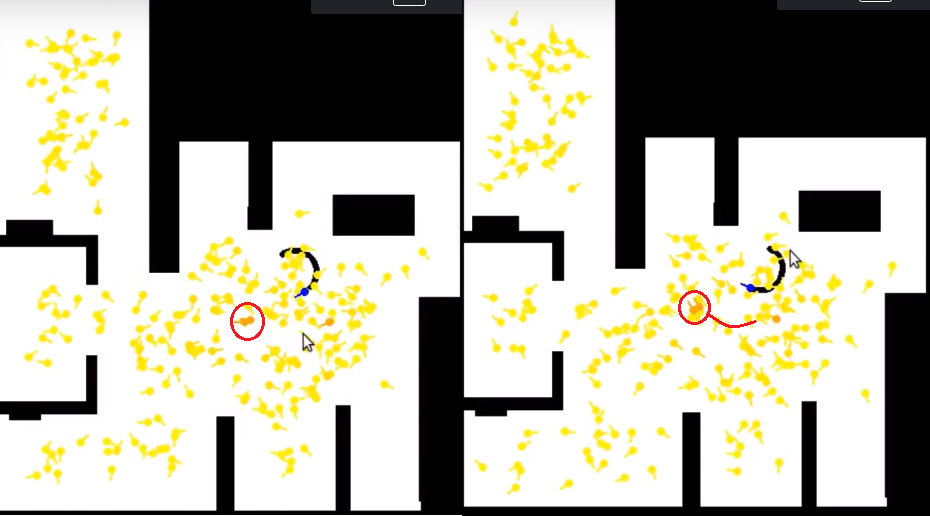
\includegraphics[width=0.65\textwidth]{figures/movimientoincorporado.png}
	\caption{Incorporación relativa de odometría}
	\label{fig.movimientoincorporado}
	\end{center}
\end{figure}

Para hacer evolucionar el conjunto hacia nuevas generaciones de partículas de manera que converjan a la posición del robot se emplea el algoritmo de la ruleta. Para ello, se acumula la probabilidad de toda la generación $Pac(x_{i}) = P(x_{i})+Pac(x_{i-1})$, y luego se asocia a cada partícula un sector cuyo ancho es proporcional a la probabilidad individual de la partícula. El girar la ruleta se materializará a través de la obtención de un número aleatorio, el cual formará parte de un único sector dentro de la ruleta, saliendo a relucir la partícula que generará descendencia (Figura 5.18). Las partículas que tienen alta probabilidad producen “picos” en la probabilidad acumulada, y por lo tanto tendrán más opciones de ser elegidas a la hora de muestrear. Así, una misma partícula puede tener muchos o hijos, o ninguno.

\begin{figure}[H]
\begin{center}
	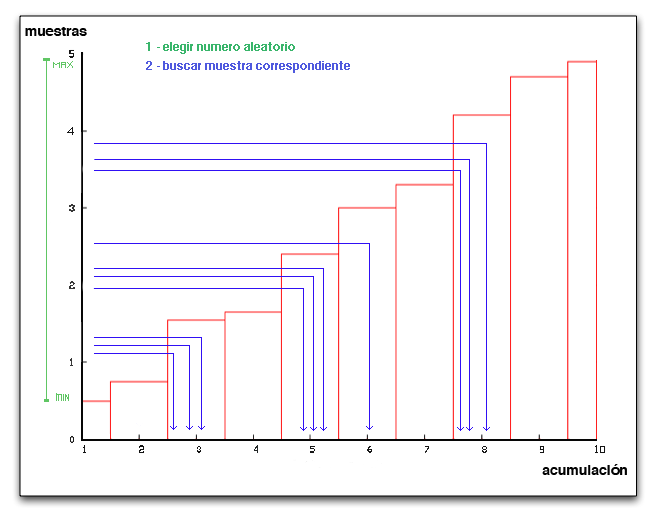
\includegraphics[width=0.65\textwidth]{figures/pacruleta.png}
	\caption{Algoritmo de la Ruleta y probabilidad}
	\label{fig.pacruleta}
	\end{center}
\end{figure}

Se evoluciona de manera más inteligente si se aplican además algunas modificaciones, como el elitismo o el ruido térmico. Una vez seleccionado el progenitor, hemos aplicado técnicas elitistas que persiguen conservar características de unas generaciones a otras preservando aquellas partículas de mayor probabilidad, distinguiendo y conservando la “élite” y eliminado las partículas que no aportan información. Así, si la partícula seleccionada para generar descendencia tiene una probabilidad muy superior a un umbral prestablecido, se copia en la siguiente generación, si su valor es ligeramente superior al umbral, se aplica un ruido térmico (gaussiano) de posición y orientación centrado en el progenitor para generar el hijo y si no supera el umbral se lanza una nueva partícula aleatoria, como al inicio del algoritmo. Esto permite también explorar los alrededores de las partículas que acumulan mayor probabilidad, pudiendo así encontrar partículas de mayor calidad en cada generación. Esto también aplica en el cálculo de la probabilidad acumulada, ya que si ésta no supera un umbral, se considera que no aporta información y se descarta la generación entera, remuestreando con una nueva generación aleatoria.

\subsection{Solución desarrollada}
En la solución de referencia desarrollada se han utilizado poblaciones de 650 partículas distribuidas por la escena, para cada una de las cuales se debe calcular 9 haces láser teóricos para asociarles una probabilidad, procesando en cada una la imagen del mapa en función de su posición. Estos valores de compromiso permiten su uso en aplicaciones en tiempo real. El utilizar 9 haces por láser en lugar de los 180 disponibles se debe a que este número de haces es suficiente para obtener lecturas representativas del entorno en cualquier punto, de manera que todos los otros rayos sólo aportarán en casos muy extremos, pero generalmente ralentizarán en gran medida el comportamiento del algoritmo y reducirán su eficiencia. 

También el hecho de segmentar la funcionalidad de la práctica en tres hilos de ejecución se debe a esto, ya que existían distintas tareas que se podían realizar de manera concurrente y compatible, ya que ninguna de ellas se cruza con las demás (toma de datos de sensores, interfaz gráfico y algoritmo).
Por otro lado, también se han precomputado todos los datos posibles para aumentar la eficiencia al máximo en cada iteración.

\subsubsection{Inicialización}
Para comenzar el algoritmo, si no se ha establecido generación de partículas se utiliza el método \textit{sendParticles()} para establecerlas de la manera aleatoria inicial. Este método se encarga de todo lo necesario para obtener una primera generación, incluyendo el trazado de rayos de cada partícula para la obtención de su láser teórico con \textit{doRayTracing()}. Hay involucradas otras funciones que comprueban si el color de un pixel es blanco o negro (\textit{isWhitePixel()}), que realizan el análisis de la información láser (\textit{parse\_laser\_data()}) y otras como el método \textit{uniform} de la biblioteca random para obtener las posiciones aleatorias entre otras. El trazado de rayos genera una lectura láser teórica del siguiente modo:

\begin{figure}[H]
\begin{center}
	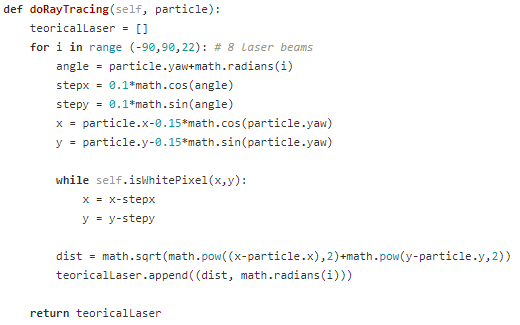
\includegraphics[width=0.65\textwidth]{figures/doraytracing.png}
	\label{fig.doraytracing}
	\end{center}
\end{figure}

\subsubsection{Modelo de observación}
Para asignar una probabilidad a cada partícula interviene el modelo de observación, el cual se invoca a través de \textit{calculateProb()}. El valor de probabilidad se asignará en función de los parecidos existentes entre cada par de haces homólogos de los laseres real y teórico, en otras palabras, se realizará una comparación haz por haz de ambos láseres. Se evalua la diferencia de distancia existente entre el haz real y el teórico en cada orientación, generando un error acumulado de distancia. Mediante este error mediremos el parecido de ambos laseres y asignaremos una probabilidad. Para ello se tiene la función que conforma el propio modelo de observación, que se ha ajustado hasta obtener resultados adecuados para esta aplicación. Se trata de una función definida a trozos de la siguiente forma:

\begin{figure}[H]
\begin{center}
	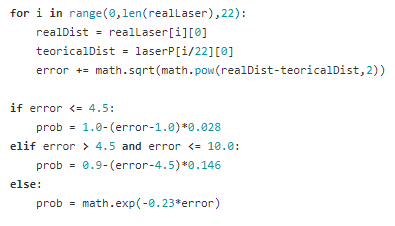
\includegraphics[width=0.65\textwidth]{figures/codemodeloobservacion.png}
	\label{fig.codemodeloobservacion}
	\end{center}
\end{figure}   

\subsubsection{Modelo de movimiento}
Lo siguiente es la incorporación de la odometría a través del modelo de movimiento, donde se actualizan todas las partículas y se gestiona si el movimiento incorporado invalida alguna partícula (tras el movimiento, algunas partículas pueden quedar fuera de los límites del espacio libre), en cuyo caso se genera una nueva partícula aleatoria. Esta incorporación es relativa a la posición y orientación de cada partícula. En este punto tendremos algo similar a la Figura 5.19:

\begin{figure}[H]
\begin{center}
	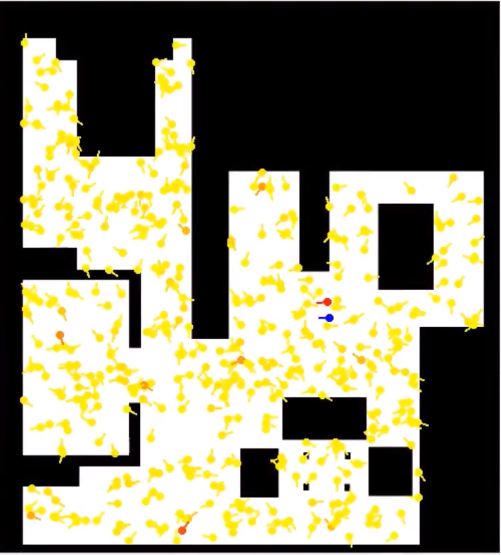
\includegraphics[width=0.45\textwidth]{figures/primerageneracion.png}
	\caption{Primera generación de partículas}
	\label{fig.primerageneracion}
	\end{center}
\end{figure}  

\subsubsection{Generación de la siguiente población}
Tras esto, es el momento de evolucionar a nuevas generaciones, si procede (con \textit{calculateNewGeneration()}). En todas las iteraciones no se realiza el cálculo de nuevas generaciones, ya que esto consumiría toda la capacidad del procesador. En base a distintas pruebas realizadas, hemos decidido implementar un reloj de generación, que evolucionará generaciones cada 300ms.
Si se trata de una \textit{iteración de generación}, los siguientes pasos son:

\begin{itemize}
	\item[--] Comprobar si la generación converge. Para ello seleccionamos la partícula de mayor probabilidad de la generación y calculamos la distancia euclidiana entre esta y cada una de las otras partículas. Si todas ellas se encuentran comprendidas en una circunferencia de radio 2m, se considera que la generación converge, y es hora de hacer una estimación con la partícula de mayor probabilidad.
	\item[--] En caso de no convergencia, y teniendo en cuenta las técnicas elitistas, en cada nueva generación se comprueba si la partícula más probable supera el 99\% de coincidencia, en cuyo caso también se crea una nueva estimación de posición.
	\item[--] En el resto de casos se calcula una nueva generación a partir de la anterior, calculando en primer lugar la probabilidad acumulada como la suma de todas las probabilidades, luego ejecutando el algoritmo de la ruleta una vez por cada nueva partícula que se quiera generar, en nuestro caso 650 veces, y con la partícula seleccionada se haga el filtro de partícula correspondiente (a través de \textit{particlesFilter}).
	\item[--] Se ha diseñado este filtro para que aplique las técnicas de selección, el ruido gaussiano y el remuestreo cuando proceda, en función de la salud de la partícula.
	\item[--] En todo caso, tras una estimación se crea una nueva generación aleatoria.
	\item[--] Habrá iteraciones de generación en las que no se haga ninguna estimación.
	\item[--] Hay condiciones de parada, como un número máximo de iteraciones de generación sin estimación, para descartar datos que no llevan a una estimación correcta. 
\end{itemize}

\section{Experimentación}
La funcionalidad descrita en los apartados anteriores ha sido ajustada a través de experimentos realizados para poner a prueba cada una de las partes. También se han hecho pruebas globales que validan experimentalmente a todo el conjunto: la infraestructura de la práctica, el nodo académico y la solución desarrollada.

\subsection{Ejecución típica}
Se ha preparado un documento de texto plano (\textit{README.md}) que sirve de guía para que alumno esté guiado durante la ejecución y el testeo, que incluye también información del API de utilización, e incluso una referencia a un vídeo demostrativo. 

La forma de ejecutar la práctica basada en interfaces de ROS es la siguiente:

\begin{enumerate}
	\item Empleamos un primer terminal para ejecutar el componente que lanza un mundo Gazebo basado en componentes de ROS:
	\begin{figure}[H]
		\begin{center}
			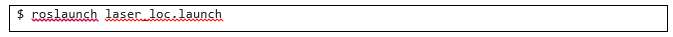
\includegraphics[width=0.95\linewidth]{figures/llcomando1.png}
			\label{fig.llcomando1}
		\end{center}
	\end{figure}
	\item Utilizamos un segundo terminal para iniciar el componente académico:
	\begin{figure}[H]
		\begin{center}
			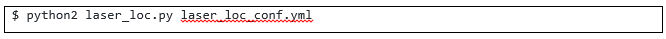
\includegraphics[width=0.95\linewidth]{figures/llcomando2.png}
			\label{fig.llcomando2}
		\end{center}
	\end{figure}
\end{enumerate}

Pulsando sobre el botón “Play Code” se podrá ver el resultado de la ejecución del algoritmo. Ejemplos de la ejecución pueden encontrarse en \footnote{\url{https://www.youtube.com/watch?v=FmUN_tzM9MM}} y \footnote{\url{https://www.youtube.com/watch?v=4OFljaeag_I}}.

\subsubsection{Localización estática}
A continuación, una serie de capturas de una ejecución representativa (Figura 5.20),

\begin{figure}[H]
	\begin{center}
		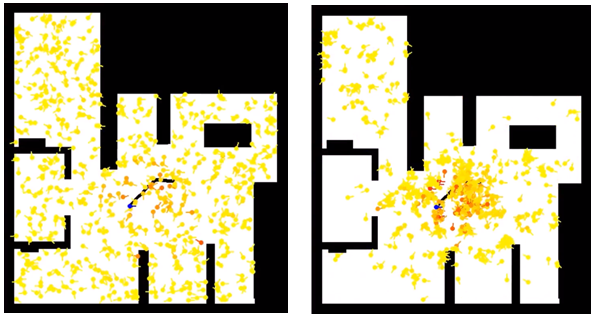
\includegraphics[width=0.850\textwidth]{figures/lloutput1.png}
		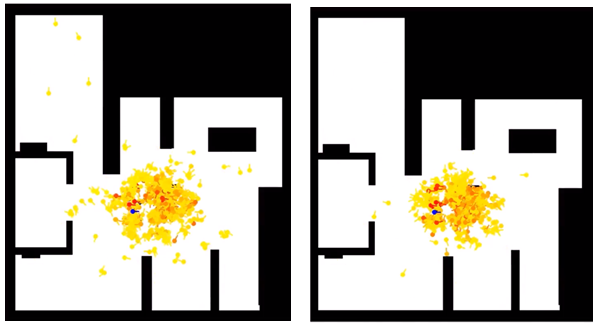
\includegraphics[width=0.850\textwidth]{figures/lloutput2.png}
		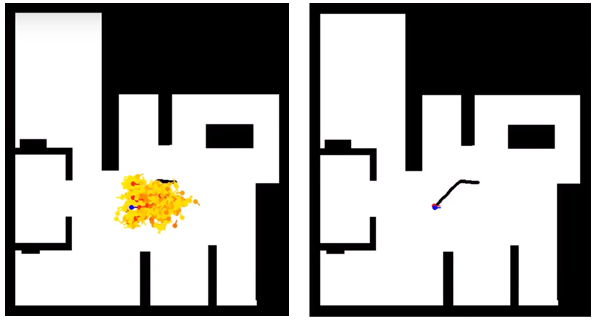
\includegraphics[width=0.850\textwidth]{figures/lloutput3.png}
		\caption{Evolución del algoritmo de localización en una ejecucion típica}
		\label{fig.outputll}
		\end{center}
\end{figure}

En este ejemplo, el robot (representado por el punto azul oscuro) permaneció estático. Se puede ver en la primera captura como la generación inicial es aleatoria, dentro de los límites de la habitación. Las siguientes 4 capturas muestran como la nube de partículas va convergiendo hacia la posición real del robot, siendo que en cada iteración la probabilidad acumulada es mayor y, por tanto, hay más partículas con alta probabilidad de ser la posición real. En la última captura se puede ver la estimación que realiza el robot una vez la generación converge en una circunferencia de radio dos.

\subsubsection{Localización en movimiento}
Al moverse el robot, no sólo se debe gestionar la comunicación con sus interfaces, sino que también se envían órdenes al interfaz para el teleoperador, para repintar el robot en el mapa, para actualizar la trayectoria y para añadir el modelo de movimiento a las partículas. Gracias al tiempo de evolución y a la programación multihilo esto es posible de manera simultánea. La localización con movimiento implicado es una manera de poner a prueba el algoritmo en un caso complejo.

Salvando fallos iniciales en algunas ejecuciones (estimaciones erróneas por algunos metros en las primeras iteraciones, pero tolerables al principio de la ejecución), los errores de posición estimada obtenidos no superan en ningún caso los 20cm, siendo la media de menos de 10cm (Figura 5.21):

\begin{figure}[H]
	\begin{center}
		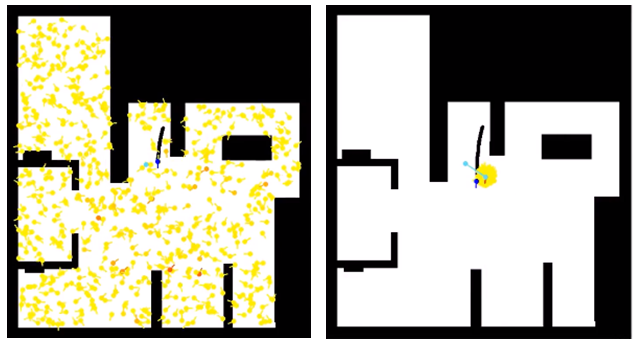
\includegraphics[width=0.850\textwidth]{figures/lloutputmov1.png}
		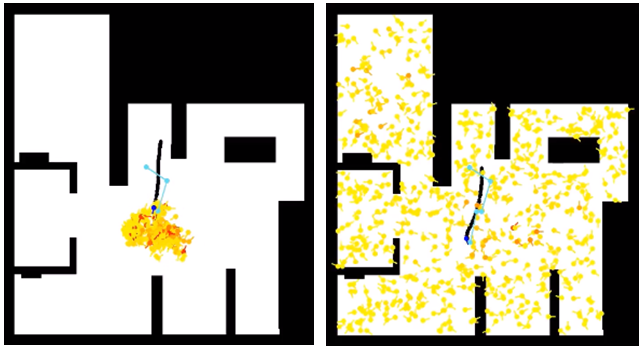
\includegraphics[width=0.850\textwidth]{figures/lloutputmov2.png}
		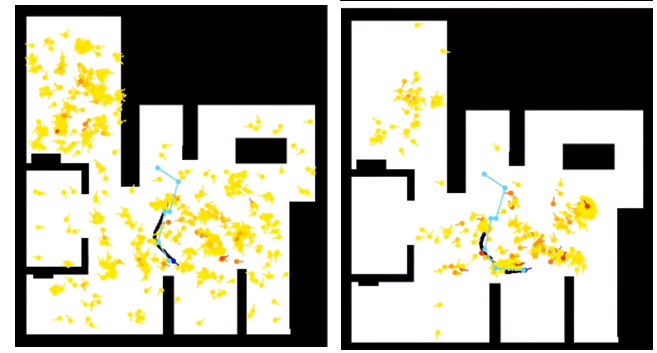
\includegraphics[width=0.850\textwidth]{figures/lloutputmov3.png}
		\caption{Evolución del algoritmo de localización con el robot moviéndose}
		\label{fig.outputllmov}
		\end{center}
\end{figure}

Estas capturas representan distintos instantes temporales, en cada uno de los cuales se ha realizado una nueva estimación de posición. Así, mientras el robot está siendo teleoperado (generando la trayectoria representada en negro) el algoritmo actúa para obtener estimaciones que la interfaz conectará entre sí, generando una trayectoria estimada (representada en azul claro). El algoritmo funciona del mismo modo, agrupando la generación en torno a la posición real, y con cada estimación se reinicia de modo aleatorio para obtener la siguiente. Algunas de estas capturas muestran un momento de agrupación, y otras un instante de reinicio.

\subsection{Autolocalización en situaciones extremas}
Decidimos poner a prueba el algoritmo en condiciones complejas (simetrías, cercanía a paredes, etc.), para comprobar si la solución propuesta era lo suficientemente buena como para lidiar con los problemas que podían surgir en entornos reales.

Aunque los escenarios simulados están compuestos por elementos de distinta naturaleza, en muchas ocasiones se tienen espacios concretos con una geometría similar (Figura 5.22), que para el ojo humano es claramente distinguible, pero no así a priori para los sensores que puede incorporar un robot.


\begin{figure}[H]
	\begin{center}
		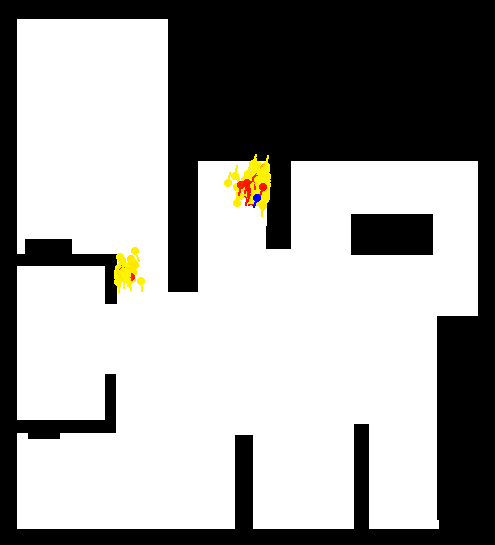
\includegraphics[width=0.59\textwidth, ]{figures/similar.png}
		\caption{Espacios de geometría similar y zonas con simetrías}
		\label{fig.similar}
		\end{center}
\end{figure}
En las pruebas realizadas en escenarios con estas simetrías, tras unas cuantas iteraciones se forman una serie de frentes de partículas que acumulan una probabilidad similar (tantos como lugares con geometría parecida existan en el entorno). Ante casos como éste, el algoritmo de localización necesitó bastantes más iteraciones de evolución de generaciones (al menos el doble en la mayoría de los casos), pero en el 70\% de ellos la estimación final venía del grupo situado en la posición correcta, es decir, en los alrededores del robot, como demuestra el punto azul celeste de la Figura 5.23).

\begin{figure}[H]
	\begin{center}
		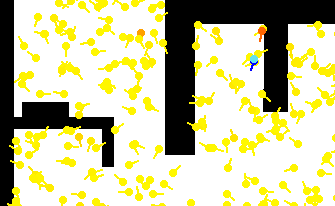
\includegraphics[width=0.4\textwidth]{figures/similaroutput.png}
		\caption{Estimación en espacios similares}
		\label{fig.similaroutput}
		\end{center}
\end{figure}

Normalmente, estos problemas de simetría se solucionan añadiendo algún otro sensor que ayude a descartar unos datos frente a otros, o simplemente incorporando movimiento, pues las posibles similitudes se irán desvaneciendo a medida que el robot avance.

Por otro lado, quisimos ver qué sucedía en caso de situar al robot muy cerca de las superficies límite (de los obstáculos). En estos casos (Figura 5.24), el robot obtiene muchos puntos en los que podría obtener una lectura dentro de los márgenes de similitud con la lectura real, de manera que se generan muchos grupos de partículas, que pueden evolucionar favorablemente o no, dependiendo de cómo fuese la distribución aleatoria inicial (recordemos que las sucesivas generaciones surgen siempre de alguna partícula preexistente). Este experimento confirmó que un algoritmo de localización robusto conviene que use datos de distintos sensores: puede basarse en láser pero ayudaría si incorporase por ejemplo información de textura para lidiar con esto.

\begin{figure}[H]
	\begin{center}
		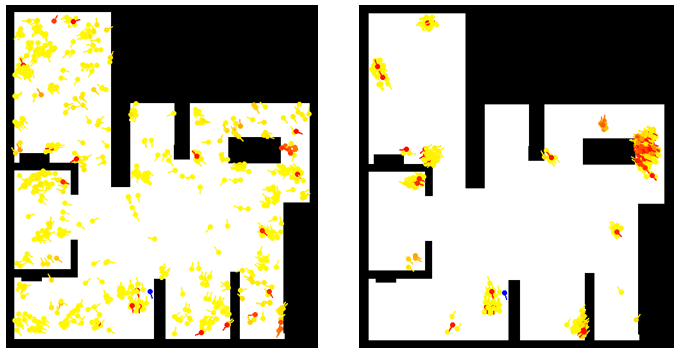
\includegraphics[width=0.88\textwidth]{figures/estampado.png}
		\caption{Posición cercana a los obstáculos}
		\label{fig.estampado}
		\end{center}
\end{figure}

Por último, sabiendo que en la realidad se dan muchos espacios simétricos (salas cuadradas, mobiliario rectangular,…), quisimos hacer un experimento en un entorno altamente simétrico, para lo cual sirvió el modelo explicado en 5.2.3, el cual es cuadrado y sólo incorpora algunos elementos que pueden generar lecturas distintas en algunos puntos (Figura 5.25):

\begin{figure}[H]
	\begin{center}
		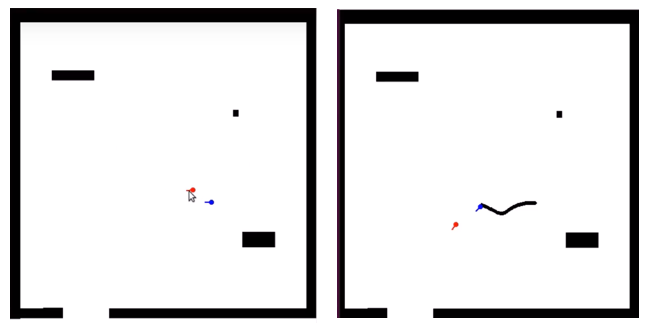
\includegraphics[width=0.88\textwidth]{figures/outputsimetrico.png}
		\caption{Estimación de autolocalización en entorno altamente simétrico}
		\label{fig.outputsimetrico}
		\end{center}
\end{figure}

El algoritmo continuó funcionando y realizando estimaciones de posición, aunque éstas en muchos casos empezaban a obtener errores más elevados, en torno a los 10-15 cm. En muchas ocasiones, estos errores pueden verse incrementados por el error que se haya cometido en el modelado del mapa, pero en cualquier caso el factor más influyente es la simetría, que al ser notable puede traducirse en distintos puntos de la sala con lecturas muy parecidas. La generación inicial aleatoria influirá en el error cometido, y por tanto la localización varía aunque se trate del mismo punto en distintas ejecuciones. En cualquier caso, las pruebas realizadas consiguieron localizar al robot cometiendo un error al límite de lo tolerable.

\subsection{Ajuste del modelo de observación}
Para alcanzar la solución se ha pasado por un proceso de ajuste de cada módulo de manera independiente. Para ajustar el modelo de observación láser empleado, y que las probabilidades que asigne se adecúen a la escena, se han usado distintos métodos:
\vspace{4cm}

\textbf{Malla de partículas}

\begin{figure}[H]
	\begin{center}
	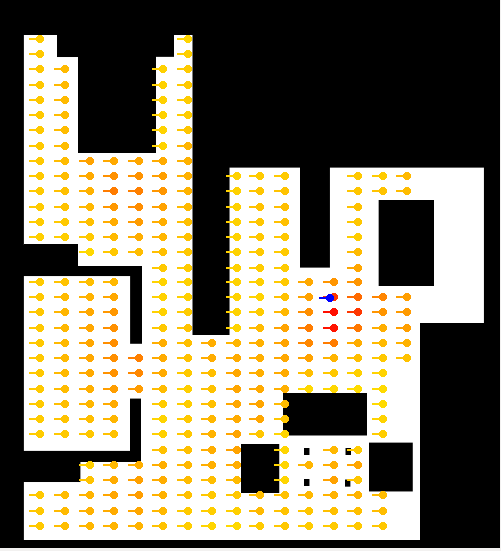
\includegraphics[width=0.55\textwidth]{figures/mallaparticulas.png}
	\caption{Malla de partículas}
	\label{fig.mallaparticulas}
	\end{center}
\end{figure}
Se trata de crear una especie de rejilla de partículas (Figura 5.26), de manera que se puede ver de forma gráfica y sencilla la distribución de la probabilidad. Para partículas cercanas al robot, las representaciones asociadas deben tomar un color más rojo, mientras que las lejanas deben tirar más hacia el amarillo. Jugando con la separación entre partículas obtuvimos la función del modelo de observación idónea para el tipo de comparación implementado entre el láser real y el teórico.

\vspace{0.5cm}
\textbf{Slider de Orientación de partículas}

De manera análoga a lo anterior, se incluyó un slider (Figura 5.27) que permitía controlar la orientación de todas las partículas al unísono y recalcular su probabilidad tras el cambio.

\begin{figure}[H]
	\begin{center}
	
\includegraphics[width=0.40\textwidth]{figures/slider.png}
	\caption{Slider de orientación}
	\label{fig.slider}
	\end{center}
\end{figure}

Esto permitió ajustar en mayor medida el modelo concreto de observación, ya que partículas en posición cercana y orientación similar (con variaciones entre 0º y 10º) deben tener una probabilidad alta, pero en posiciones similares y orientaciones distintas (>20º) deben tener probabilidades bajas (Figura 5.28).

\begin{figure}[H]
		\begin{center}
		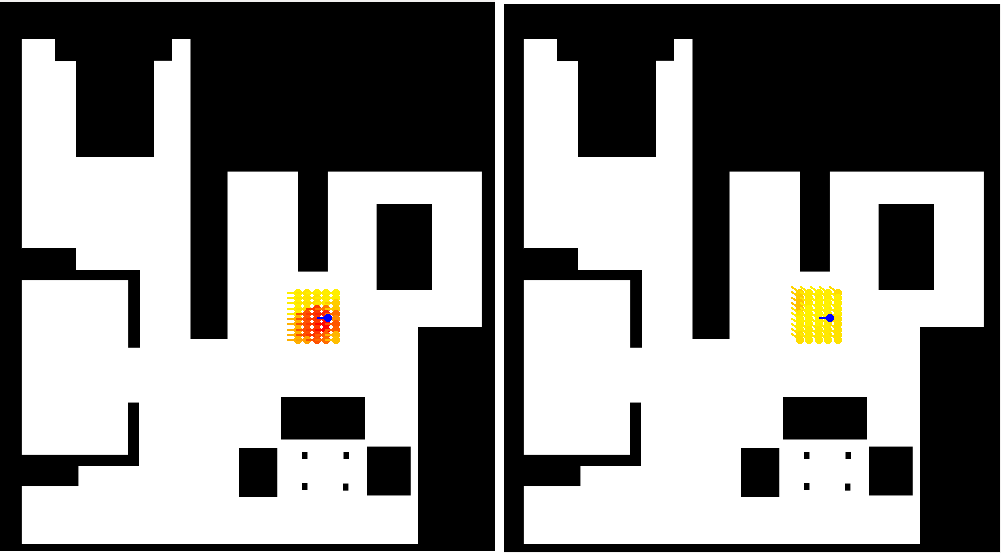
\includegraphics[width=0.85\textwidth]{figures/slidermap.png}
		\caption{Ajuste de Modelo de Observación (diferencia angular de 0º vs. diferencia angular de 40º con la orientación real)}
		\label{fig.slidermap}
		\end{center}
	\end{figure}
	
\subsection{Ajuste del Ruido Gaussiano en la generación de nuevas partículas}
Para llevar a cabo la exploración de una zona en la que existe una partícula de alta probabilidad, la descendencia de la misma se crea añadiendo un pequeño ruido que no debe dispersar demasiado las nuevas partículas generadas, ya que la intención es encontrar una nueva posición más favorable, la cual tiene altas probabilidades de estar muy cerca y en una orientación muy parecida. Se probó con diferentes configuraciones de ruido, para al final decantarnos por una distribución normal centrada en la posición del progenitor con una desviación típica $\sigma$ de 0.1.

\subsection{Ajuste del tiempo de evolución de las partículas}
Ya se ha mencionado que las generaciones no se evolucionan en todas las iteraciones del algoritmo, sino que se ha establecido un tiempo de evolución. El ajuste de este tiempo se basado en la rapidez del algoritmo en proporcionar una estimación: de media han sido necesarias 13 generaciones para obtener una estimación, y en vistas a lograr la localización de un robot en movimiento, se decidió que era necesaria al menos 1 estimación cada 4 segundos, de manera que se fijó dicha evolución en intervalos de 300 ms. 

\section{Cuadernillo Jupyter Académico}
Esta práctica lleva mucha más carga y complejidad gráfica que la descrita en el Capítulo 4, de manera que hemos tenido que explorar las opciones de interfaz gráfica que ofrece Jupyter. Aunque permite lanzar subprocesos desde los \textit{Notebooks}, la idea que nos ha resultado más atractiva ha sido la de construir \textit{widgets} interactivos, controlados por código Python, a través de bibliotecas de representación como \textit{MatPlotLib}, que recogen eventos de usuario y los materializan en la funcionalidad necesaria, permitiendo así disponer de una interfaz gráfica en el cuadernillo. Con estos nuevos integrantes sumados a los que ya habíamos empleado (celdillas de código, imágenes, texto con formato, etc.) hemos preparado un cuadernillo de Jupyter al que hemos llamado \textit{laser\_loc.ipynb} (Figura 5.29), a través del cual accederemos a la versión de Jupyter de esta práctica. 

En esta ocasión, los cambios en el nodo son mayores que en el ejercicio anterior, dado que es necesario gestionar toda la funcionalidad de interacción desde el mismo, y además construir la forma de comunicación entre el cuadernillo y el \textit{kernel} de Jupyter. En concreto, el nodo programado en el fichero \textit{lase\_loc.py} de la práctica original ha sido recodificado para tener estructura de clase Python (\textit{LaserLoc}), a la cual le hemos incorporado todos los atributos y métodos necesarios tanto para el soporte de la práctica como para su parte gráfica. 

\begin{figure}[H]
	\begin{center}
		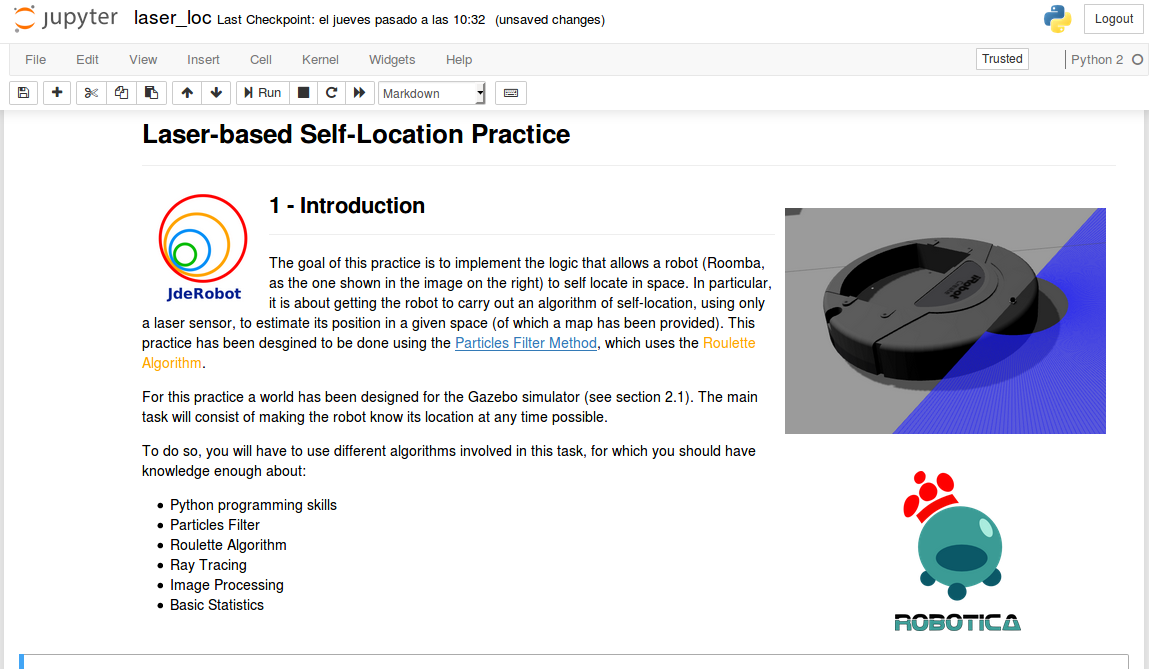
\includegraphics[width=0.98\textwidth]{figures/laserlocjupyter.png}
		\caption{Cuadernillo del ejercicio de localización por filtro de partículas}
		\label{fig.laserlocjupyter}
		\end{center}
\end{figure}

Aunque los elementos principales del \textit{Notebook} son los \textit{widgets} interactivos y las celdas de código, también se ha incluido texto de apoyo para los pasos a seguir en la resolución de la práctica e imágenes representativas de las salidas que se pueden ir obteniendo, todo lo cual creemos que es de gran ayuda para orientar al alumno, en especial, la descripción del API de funcionalidad que la clase \textit{LaserLoc} del cuadernillo pone a su disposición.

En cuanto a los elementos interactivos, hemos incluido principalmente dos dinámicos y uno estático basados en los que ya había en la interfaz de la versión de escritorio de la práctica. El \textit{widget} del teleoperador (Figura 5.30) no es más que una representación básica de dos rectas sobre un fondo negro. Sin embargo, ha sido preparado para recoger eventos del ratón desde la aplicación (\textit{press} y \textit{release}), y para enviar órdenes a los actuadores del robot en función de estos y que se reflejen en la simulación. Así, si el usuario hace click sobre este \textit{widget}, arrastra la cruz hasta un punto determinado y deja de presionar el ratón, consigue materializar un movimiento proporcional al movimiento de la cruz en el robot. Con este elemento mantenemos la posibilidad de probar el algoritmo en condiciones de localización en movimiento. 

\begin{figure}[H]
	\begin{center}
		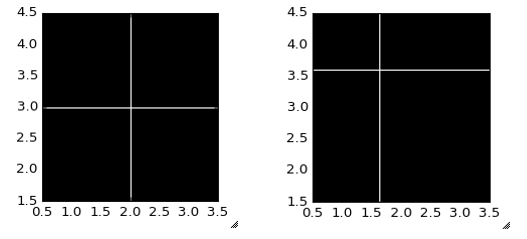
\includegraphics[width=0.68\textwidth]{figures/teleoperadorjupyter.png}
		\caption{Teleoperador en Jupyter}
		\label{fig.laserlocjupyter}
		\end{center}
\end{figure}


El \textit{widget} del mapa binario (Figura 5.31) consta de varios elementos. Como se puede ver en la Figura inferior, se han dispuesto 3 botones que también recogen la interacción. El primero (en rojo), tiene que ver con el \textit{widget} anterior, y sirve para parar el movimiento del robot y restablecer la posición del teleoperador, para facilitar el control del mismo. El segundo (en azul) es el que se utiliza para ejecutar la función \textit{cretaeNewGeneration}, una de las dos que el alumno debe implementar para alcanzar la solución. Esta función es la encargada de evolucionar las generaciones bajo la orden del alumno, con cada click genera un nuevo conjunto de partículas basado en el precedente. Por último (en verde), el botón \textit{Play Code} ejecuta el código del método \textit{execute}, el cual también debe ser codificado por el alumno, que recoge la funcionalidad principal del algoritmo, y que debe gestionar también el cálculo del láser de una posible partícula sobre la que se haga click en el mapa.

\begin{figure}[H]
	\begin{center}
		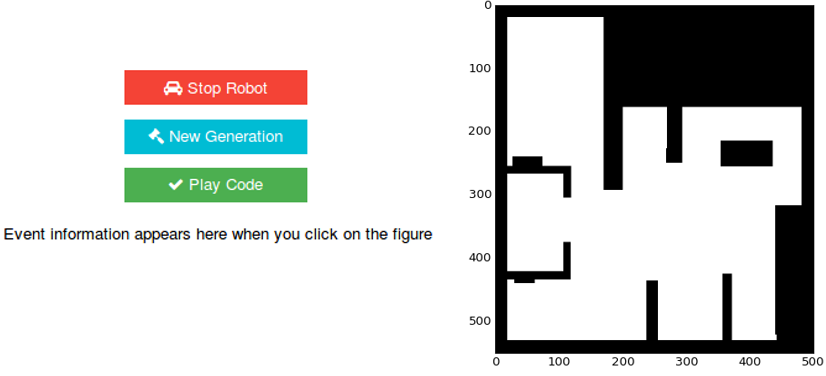
\includegraphics[width=0.90\textwidth]{figures/mapabinariojupyter.png}
		\caption{Widget de Mapa Binario en Jupyter}
		\label{fig.mapabinariojupyter}
	\end{center}
\end{figure}

El elemento principal del \textit{widget} es el mapa, que se ha extrapolado directamente desde la interfaz de la práctica, siendo una imagen binaria que permitirá visualizar la evolución del algoritmo. También es un elemento dinámico que variará cada vez que evolucione una generación, y que recogerá los clicks del usuario para traducir las coordenadas del ratón en coordenadas de una partícula y así poder realizar el cálculo de su láser y su representación.

La representación láser (Figura 5.32) es un \textit{widget} estático equivalente a la gráfica de los láseres real y teórico de la práctica original. En cuanto se hace click sobre una partícula en el mapa, si se ejecuta la celdilla de código del \textit{Notebook} indicada para la representación láser, se refresca su salida, donde el láser teórico (rojo) se superpone a los datos reales (azul). La celdilla de este elemento también mostrará por su salida la probabilidad asociada a la partícula sobre la que se ha hecho click.

\begin{figure}[H]
	\begin{center}
		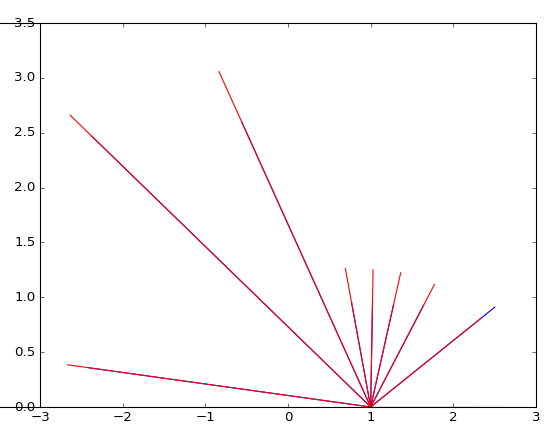
\includegraphics[width=0.49\textwidth]{figures/laserjupyter.png}
		\caption{Widget Láser en Jupyter}
		\label{fig.laserjupyter}
	\end{center}
\end{figure}

Todos estos elementos contribuyen a que la funcionalidad de la práctica esté soportada desde Jupyter, de manera que en una ejecución concreta se obtienen salidas equivalentes a los que se obtendrían fuera de esta aplicación (Figura 5.33).

\begin{figure}[H]
	\begin{center}
		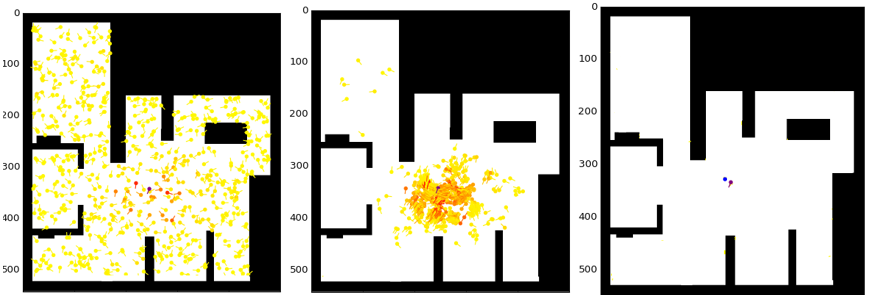
\includegraphics[width=0.99\textwidth]{figures/outputjupyterll.png}
		\caption{Evolución de una ejecución típica del ejercicio en un cuadernillo de Jupyter}
		\label{fig.laserjupyter}
	\end{center}
\end{figure}

En \footnote{\url{https://www.youtube.com/watch?v=kF7szwrC6a0}} se puede ver un vídeo demostrando el comportamiento de la práctica a través de un cuadernillo Jupyter.